\subsection{Quality at a matched time budget}
\label{sec:anytime}

\begin{figure}[tbp]
  \centering
  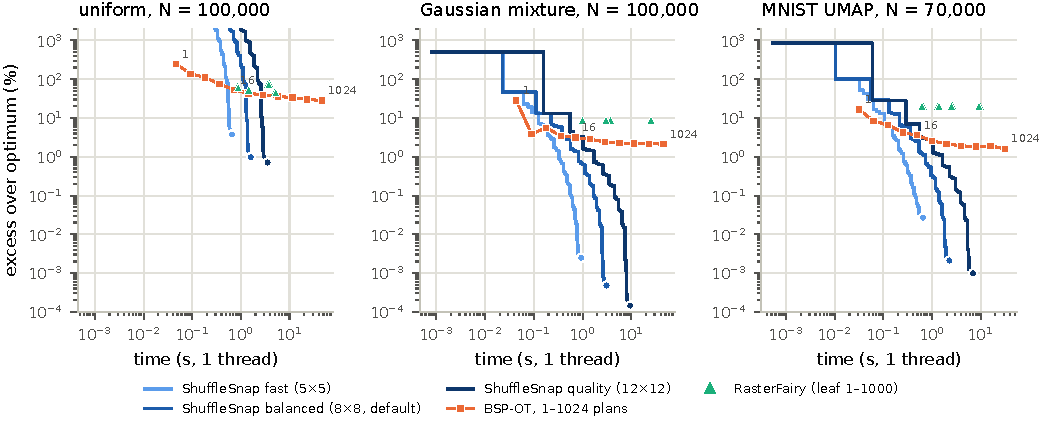
\includegraphics[width=\linewidth]{figures/fig_anytime_t1.pdf}
  \caption{Excess over the certified optimum against elapsed time, one thread. \ShuffleSnap's
  step curves record the exact cost after every phase, so each shows the result that a time
  budget ending at that moment would return. BSP-OT is run separately with 1, 2, 4, \dots,
  1024 plans (labels at 1, 16 and 1024). RasterFairy upstream is shown with exact leaf
  blocks of 1, 50, 200 and 1000 points. Instance seed 1. The same plot with 24 threads is
  in the appendix (Figure~\ref{fig:anytime24}).}
  \label{fig:anytime}
\end{figure}

Figure~\ref{fig:anytime} compares the methods at matched time budgets. BSP-OT improves
slowly with more plans and levels off far from the optimum. From 1 to 16 to 1024 plans,
its excess drops from 249\% to 53\% to 28\% on uniform points, from 28\% to 3.1\% to
2.1\% on the mixture, and from 16\% to 3.6\% to 1.6\% on MNIST. The 1024-plan runs take
31--46\,s on one thread. The \ShuffleSnap\ baseline passes that best BSP-OT result after
1.1--1.3\,s and finishes at 2.5\%, 0.004\% and 0.014\% respectively. At equal elapsed
time, \ShuffleSnap\ is ahead from 0.7--1.3\,s onward. With less time than that (on one
thread at $10^5$ points), BSP-OT is the better choice, because \ShuffleSnap\ has only
finished its coarsest levels. With 24 threads, the crossover moves to 0.04--0.09\,s.
RasterFairy's leaf size hardly matters except on uniform points (73\% with no exact leaves,
45\% with 1000-point leaves).
